% Diagrammatic notation for tensors, and what contracting an index means (Session 5).
% Own drawing. Compile with: pdflatex tensor_notation.tex ; result moves to ../tensor_notation.pdf
\documentclass[11pt,tikz,border=3pt]{standalone}
\usepackage{amsmath,amssymb}
\usepackage{xcolor}
\definecolor{coursedark}{HTML}{1B2A4A}
\definecolor{courseaccent}{HTML}{7A2E8C}

\begin{document}
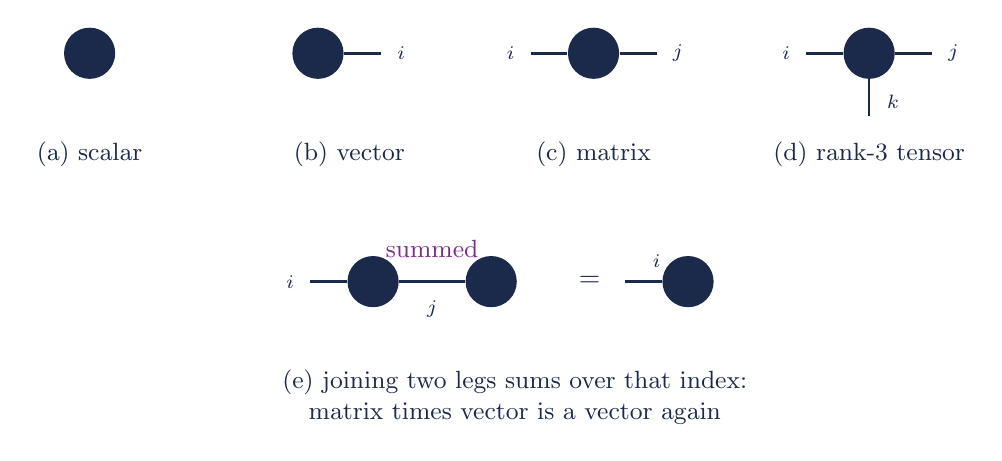
\begin{tikzpicture}[
    tensor/.style={circle, fill=coursedark, minimum size=6.5mm, inner sep=0pt},
    wire/.style={draw=coursedark, line width=0.9pt},
    lbl/.style={font=\small, text=coursedark, align=center},
    idx/.style={font=\scriptsize, text=coursedark},
  ]

  \def\leg{0.8}

  % ---------- (a) scalar
  \begin{scope}[shift={(0,0)}]
    \node[tensor] (a) at (0,0) {};
    \node[lbl, anchor=north] at (0,-1.0) {(a) scalar};
  \end{scope}

  % ---------- (b) vector
  \begin{scope}[shift={(2.9,0)}]
    \node[tensor] (b) at (0,0) {};
    \draw[wire] (b) -- ++(\leg,0);
    \node[idx, anchor=west] at (0.88,0) {$i$};
    \node[lbl, anchor=north] at (0.4,-1.0) {(b) vector};
  \end{scope}

  % ---------- (c) matrix
  \begin{scope}[shift={(6.4,0)}]
    \node[tensor] (c) at (0,0) {};
    \draw[wire] (c) -- ++(\leg,0);
    \draw[wire] (c) -- ++(-\leg,0);
    \node[idx, anchor=east] at (-0.88,0) {$i$};
    \node[idx, anchor=west] at (0.88,0) {$j$};
    \node[lbl, anchor=north] at (0,-1.0) {(c) matrix};
  \end{scope}

  % ---------- (d) rank-three tensor
  \begin{scope}[shift={(9.9,0)}]
    \node[tensor] (d) at (0,0) {};
    \draw[wire] (d) -- ++(\leg,0);
    \draw[wire] (d) -- ++(-\leg,0);
    \draw[wire] (d) -- ++(0,-\leg);
    \node[idx, anchor=east] at (-0.88,0) {$i$};
    \node[idx, anchor=west] at (0.88,0) {$j$};
    \node[idx, anchor=west] at (0.1,-0.62) {$k$};
    \node[lbl, anchor=north] at (0,-1.0) {(d) rank-3 tensor};
  \end{scope}

  % ---------- (e) contraction
  \begin{scope}[shift={(3.6,-2.9)}]
    \node[tensor] (e1) at (0,0) {};
    \node[tensor] (e2) at (1.5,0) {};
    \draw[wire] (e1) -- ++(-\leg,0);
    \draw[wire] (e1) -- (e2);
    \node[font=\small, text=courseaccent, anchor=south] at (0.75,0.18) {summed};
    \node[idx, anchor=east] at (-0.88,0) {$i$};
    \node[idx, anchor=north] at (0.75,-0.12) {$j$};
    \node[text=coursedark] at (2.75,0) {$=$};
    \node[tensor] (e3) at (4.0,0) {};
    \draw[wire] (e3) -- ++(-\leg,0);
    \node[idx, anchor=south] at (3.6,0.06) {$i$};
    \node[lbl, anchor=north] at (1.8,-1.0)
      {(e) joining two legs sums over that index:\\ matrix times vector is a vector again};
  \end{scope}

\end{tikzpicture}
\end{document}
